\documentclass{article}
\usepackage{amsmath}
\usepackage{amssymb}
\usepackage{graphicx}
\usepackage{witharrows}
\usepackage{caption}
\usepackage{subcaption}
\usepackage{float}

\begin{document}
\title{Homework 1}
\author{Mauro Patimo}

\maketitle

\section{Problem 1}
$f_3=f_1(t+1)+f(t-1)$ \\
\\
$f_4=f(t-\frac{1}{2})+f_1(t+\frac{1}{2})$ \\
\\
$f_5=1.5f(\frac{t}{2}-1)$
\section{Problem 2}
\subsection*{2a}
\begin{figure}[H]
    \begin{subfigure}{0.5\textwidth}
        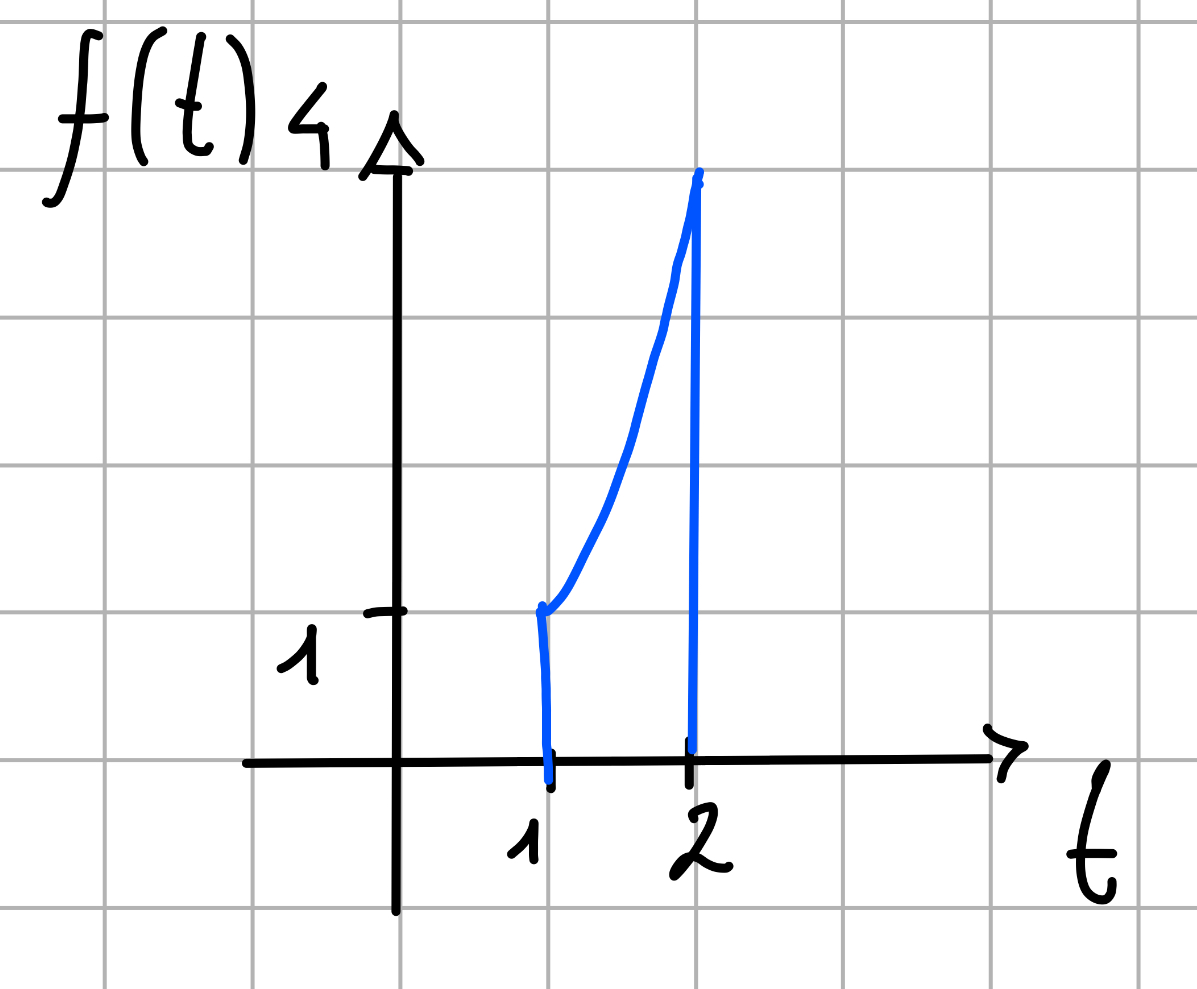
\includegraphics[width=\linewidth]{Ex_2a.jpg}
        \caption{Problem 2a}
    \end{subfigure}
    \begin{subfigure}{0.5\textwidth}
        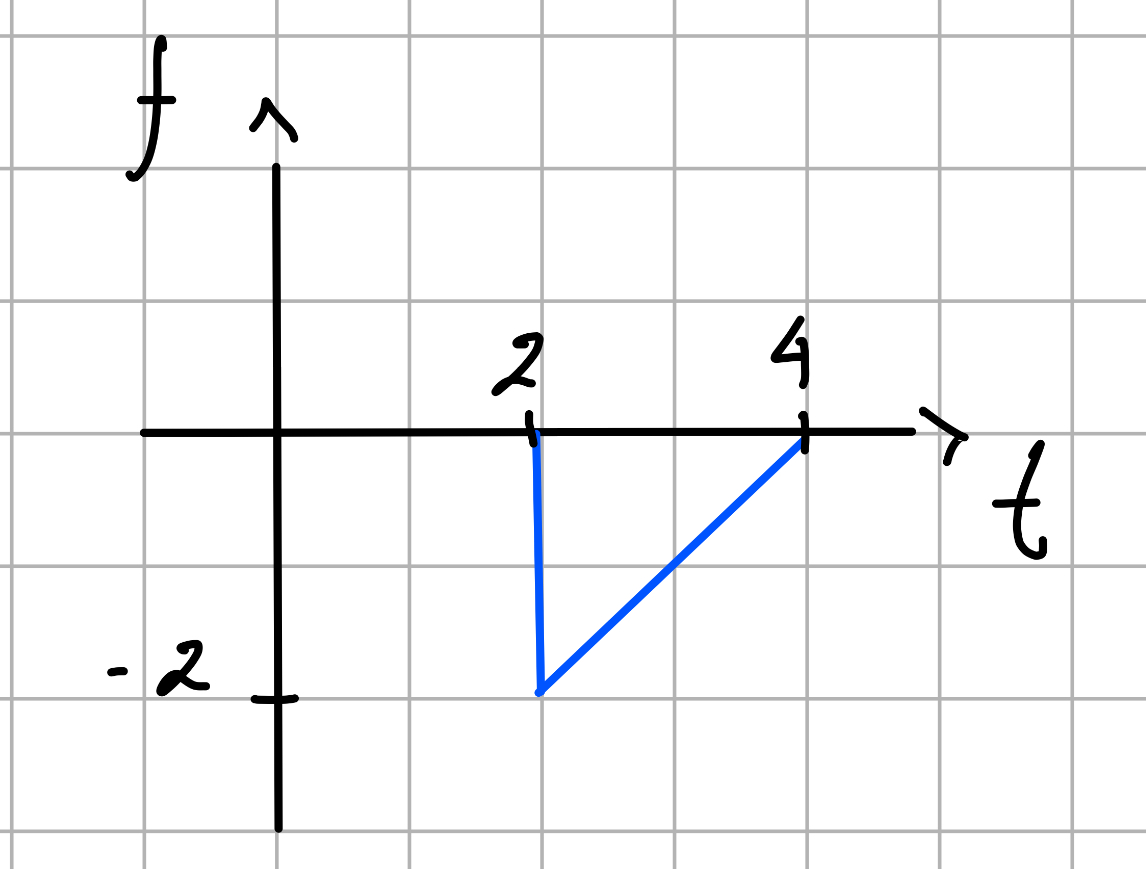
\includegraphics[width=\linewidth]{Ex_2b.jpg}
        \caption{Problem 2b}
    \end{subfigure}
    \caption{Problem 2}
\end{figure}
\section{Problem 3}
\subsection{a}
$\int_{-\infty}^{\infty}\delta (\tau)f(t-\tau)d\tau$\\ \\
$t-\tau=\alpha$ $\rightarrow$ $\tau=t-\alpha$\\ \\
$-\int_{-\infty}^{\infty}\delta (t- \alpha)f(\alpha)d\alpha$\\ \\
Since $\delta (-\alpha)=\delta (\alpha)$\\ \\
$-\int_{-\infty}^{\infty}\delta(-\alpha-(-t))f(-\alpha)$ \\ \\
$-\alpha=\sigma$ \\ \\
$-\int_{-\infty}^{\infty}\delta(\sigma-(-t)t)f(\sigma)d\sigma$ \\ \\
$f(\sigma)=f(-\alpha)=f(t-\tau)$
\subsection{b}
$\int_{-\infty}^{\infty}\delta(t+3)e^{-t}dt$\\ \\
$e^{3}$
\subsection{c}
$\int_{-\infty}^{\infty}f(\tau)\delta(t-\tau)d\tau$ \\ \\
$\int_{-\infty}^{\infty}f(t)\delta(\tau-t)d\tau$
$f(t)$
\subsection{d}
$\int_{-\infty}^{\infty}f(2-t)\delta(3-t)$ \\ \\
$3-t=\alpha$ \\ \\
$\int_{-\infty}^{\infty}f(\alpha+1)\delta(\alpha)$ \\ \\
$f(-1)$
\section{Problem 4}
\subsection*{a}
$\frac{sin(0)}{0^2+2}\delta (t)=0$
\subsection*{b}
$\frac{1}{-3j+2}\delta (t+3)=\frac{1}{-3j+2}\delta (w+3)$
\subsection*{c}
$\frac{sin(0k)}{0}\delta (\omega)$ \\
$\frac{kcos(0k)}{1}\delta (\omega)=k\delta(\omega)$
\section{Problem 5}
$P=\lim_{t\to\infty}\frac{1}{T}\int_{-\infty}^{\infty}(Ccos(\omega t +\theta))^2dt$ \\ \\
$P=\frac{1}{2\pi}\int_{0}^{2\pi}(Ccos(\omega t +\theta))^2dt$ \\ \\
$P=\frac{1}{2\pi}C^2\pi$ \\ \\
$P=\frac{C^2}{2}$
\section{Problem 6}
\subsection*{a}
\begin{figure}[H]
    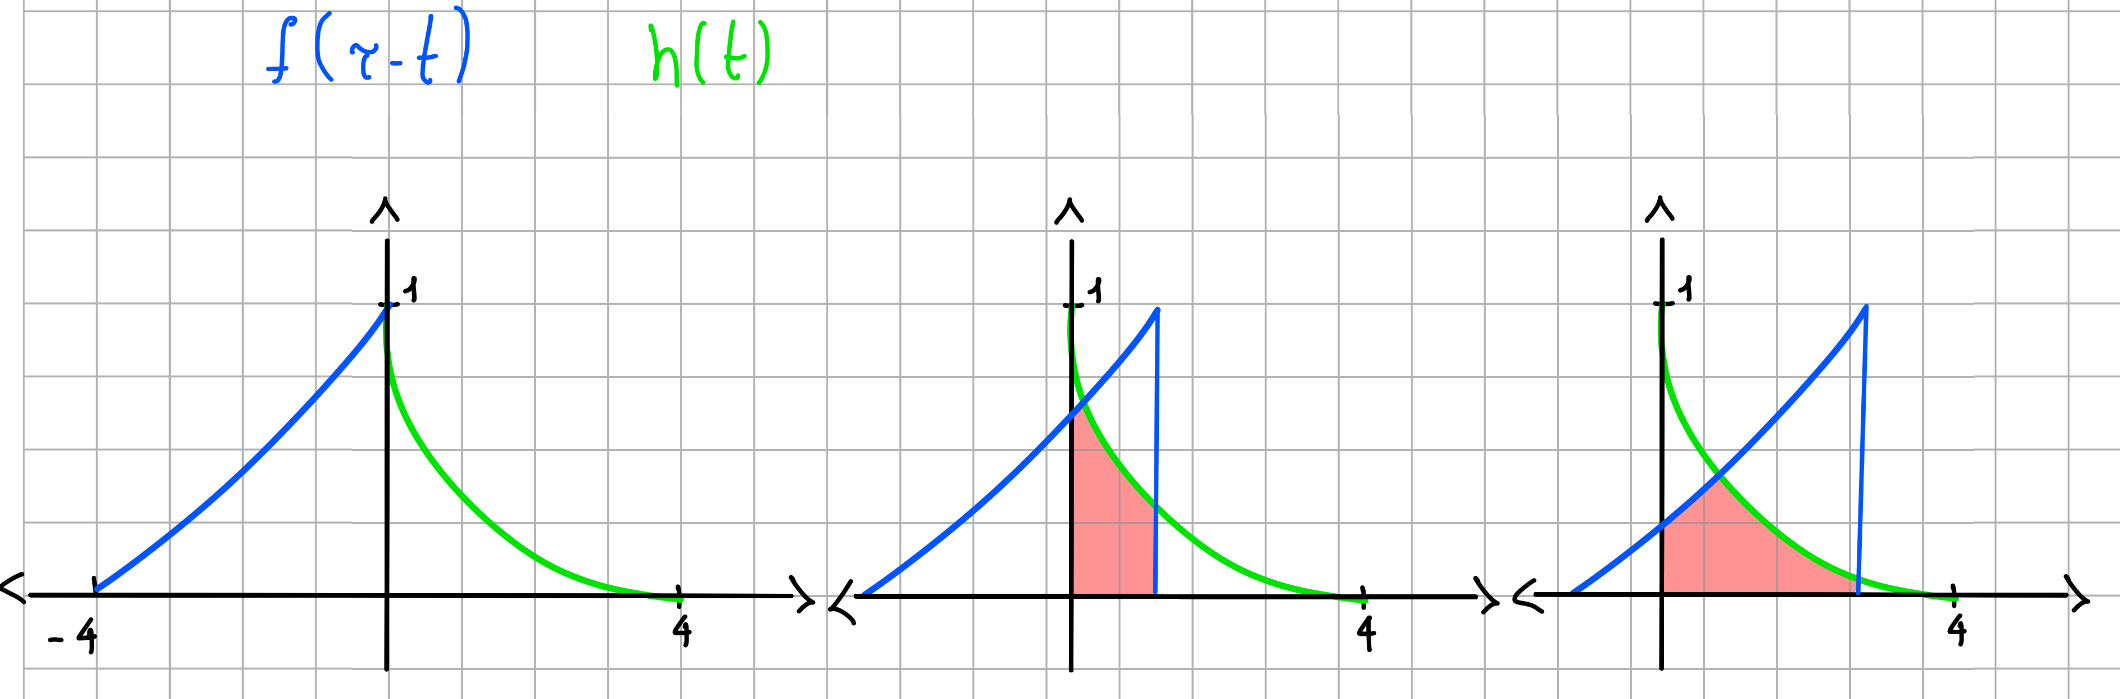
\includegraphics[width=\textwidth]{Ex_6a.jpg}
    \caption{Problem 6a}
\end{figure}
\subsection*{b}
\begin{figure}[H]
    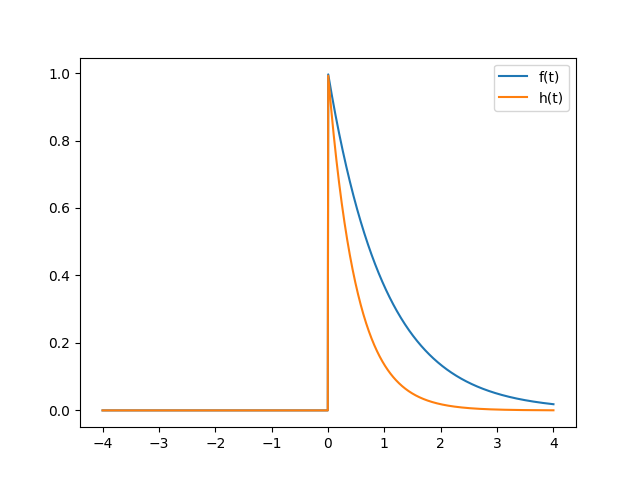
\includegraphics[width=\textwidth]{Pre-convolution.png}
    \caption{Pre-convolution}
\end{figure}
\begin{figure}[H]
    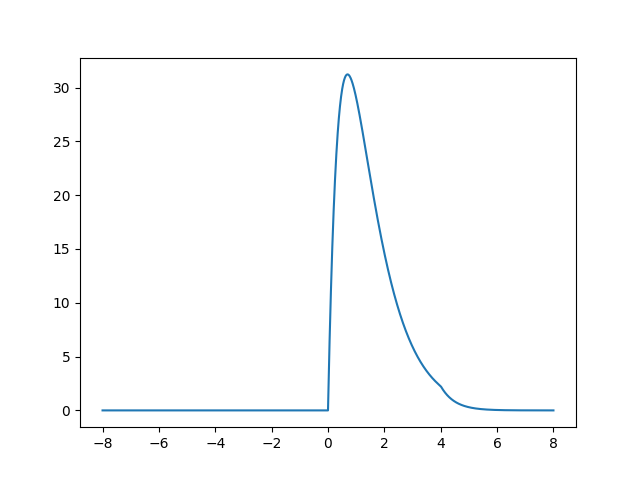
\includegraphics[width=\textwidth]{Convolution.png}
    \caption{Convolution}
\end{figure}
\title{597}
\maketitle
\section*{Problem 1}
\subsection*{a}
\begin{figure}[H]
    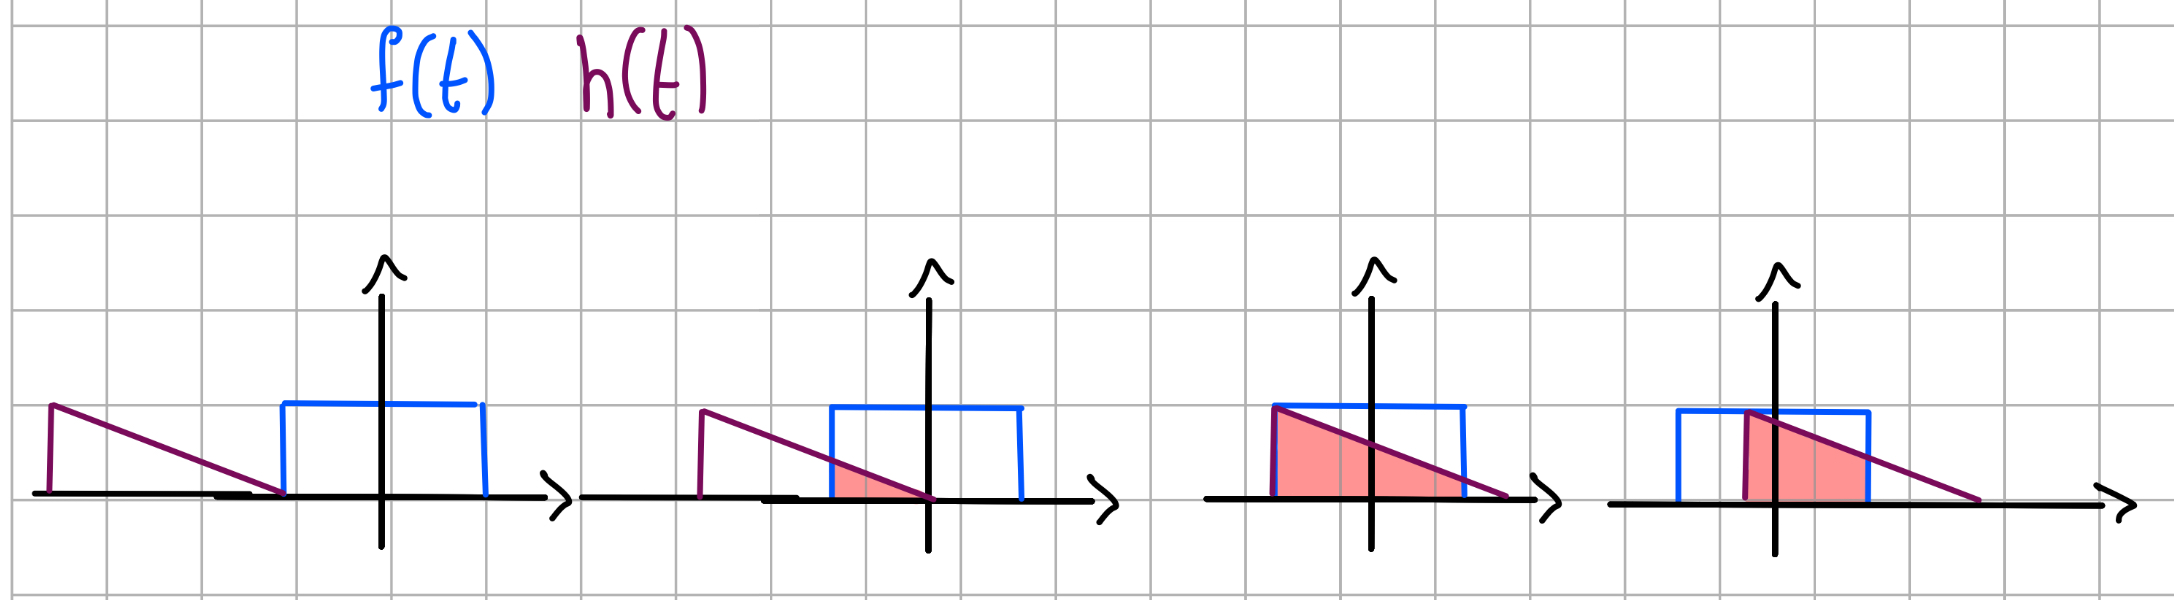
\includegraphics[width=\textwidth]{Ex_1a.jpg}
    \caption{Problem 1a}
\end{figure}
\subsection*{b}
\begin{figure}[H]
    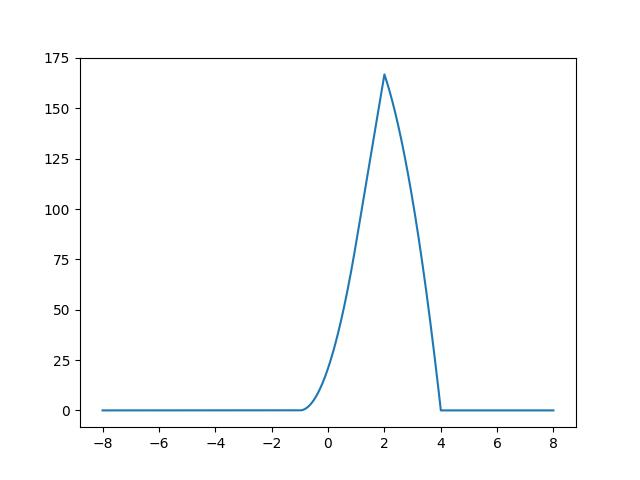
\includegraphics[width=\textwidth]{Ex_1b.jpg}
    \caption{Problem 1b}
\end{figure}
The length is 5, as expected by summing the lengths of the two functions.
\section*{Problem 2}
\subsection*{b}
$P=\frac{1}{T} \lim_{T\to\infty}\int_{-\infty}^{\infty}(f_1(t)+f_2(t))^2dt=\\
=\frac{1}{2\pi}\Big(\int_{0}^{2\pi}(C_1cos(\omega_1t+\theta_1))^2 + \int_{0}^{2\pi}(C_1cos(\omega_2t+\theta_2))^2\Big) + \frac{1}{\pi}\int_{0}^{2\pi}C_1C_2cos(\omega_1t+\theta_1)cos(\omega_2t+\theta_2)dt \\
=\frac{C_1^2}{2}+\frac{C_2^2}{2}\frac{1}{\pi}\int_{0}^{2\pi}C_1C_2cos(\omega_1t+\theta_1)cos(\omega_2t+\theta_2)dt \\ $
In case $\omega_1=n\omega_2$ where "n" is not irrational and non-zero the function is periodic. 
\subsection*{c}
As explained in part b, if $\omega_1=\omega_2$ the function is periodic. \\
\end{document}
